\documentclass[11pt, a4paper, fleqn]{article}

\usepackage[portuguese]{babel}
\usepackage{graphicx}
\usepackage{leading}
\usepackage{tabularx}
\usepackage{geometry}
\usepackage[utf8]{inputenc}
\usepackage{booktabs}
\usepackage{array}

%----------------- font -------------------------------------------------------%
\usepackage[T1]{fontenc}
\usepackage{paratype}
\usepackage[basic, italic]{mathastext}

%----------------- titles formats ---------------------------------------------%
\usepackage{titlesec}
\titleformat{\part}
{\LARGE\bfseries}{\thepart}{1em}{}
\titleformat{\section}
{\LARGE\bfseries}{\thesection}{1em}{}
\titleformat{\subsection}
{\Large\bfseries}{\thesubsection}{1em}{}
\titleformat{\paragraph}[runin]
{\sffamily\bfseries}
{}
{0pt}
{}

%----------------- footnote format --------------------------------------------%
\usepackage[perpage, bottom, marginal]{footmisc}
\makeatletter
\renewcommand{\@makefnmark}{\hbox{\textsuperscript{\sffamily\@thefnmark}}}
\makeatother
\renewcommand*{\footnotelayout}{\footnotesize\sffamily}

%----------------- page number format -----------------------------------------%
\usepackage{fancyhdr}
\fancypagestyle{pagestyle}{%
	\fancyhf{} % clear all header and footer fields
	\fancyfoot[C]{\makebox[\textwidth]{\sffamily\normalsize\thepage}} % centered footer
	\renewcommand{\headrulewidth}{0pt}
	\renewcommand{\footrulewidth}{0pt}
}

%----------------- verbatim ---------------------------------------------------%
\usepackage{fancyvrb}

\begin{document}
	\sffamily
	\setlength{\parindent}{0em}
	\emergencystretch 3em
	\renewcommand{\baselinestretch}{1.25} 
	
	\begin{titlepage}
		
\includegraphics[width=26mm]{imgs/UM.jpg}
\includegraphics[width=26mm]{imgs/EE.jpg}
		
		\vspace{7mm}
		\leading{17pt}
		{\Large
			\textbf{Universidade do Minho}
			\\
			{\fontseries{l}\selectfont
				Escola de Engenharia
		}}
		
		\vspace{50mm}
		\leading{27pt}
		{\huge
			\textbf{Inteligência Artificial}
			\\
			Trabalho Prático
		}
		\\
		%
		\\
		{\LARGE
			Licenciatura em Engenharia Informática
			\\
			Ano Letivo 2025/2026}
		
		\vspace{22mm}
		\leading{15pt}
		{\Large
			\begin{tabularx}{\textwidth}{@{}p{20mm} X}
				\multicolumn{2}{@{}l}{\textbf{Grupo 04}} \\
				\multicolumn{2}{@{}l}{} \\
				106919 & Eduardo Freitas Fernandes \\ 
				106842 & Gonçalo Rodrigues Ribeiro \\
				106888 & José Mário Raimundo Lima \\
				108961 & Rodrigo Novais da Silva
			\end{tabularx}
		}
		
		\vspace*{\fill}
	\end{titlepage}
	
	\newgeometry{left=25mm,right=20mm,top=25mm,bottom=25mm}
	\setlength{\parindent}{1em}
	
	
	\noindent \textbf{{\LARGE Avaliação por Pares}} \\
	
	\noindent A106919 Eduardo Freitas Fernandes DELTA = 0
	
	\noindent A106842 Gonçalo Rodrigues Ribeiro DELTA = 0
	
	\noindent A106888 José Mário Raimundo Lima DELTA = 0
	
	\noindent A108961 Rodrigo Novais da Silva DELTA = 0
	
	\vspace{3em}
	
	\tableofcontents
	
	\newpage
	
	
	\section{Introdução}
	
	
	Este projeto tem como objetivo o desenvolvimento de um sistema inteligente para a gestão e otimização de uma frota de táxis mista (veículos elétricos e a combustão) da empresa \textbf{TaxiGreen}.
	
	O problema central reside na alocação eficiente de veículos a pedidos dinâmicos num ambiente urbano, considerando restrições de autonomia, tempos de recarga (no caso de veículos elétricos) e preferências dos clientes (custo, rapidez ou até preferência ambiental).
	
	A solução desenvolvida modela um conjunto de zonas da cidade de Guimarães como um grafo e implementa algoritmos de procura para calcular rotas e tomar decisões de reabastecimento em tempo real.
	
	\section{Formulação do Problema}
	
	\subsection{Tipo de Problema}
	
	O problema é formulado como um \textbf{problema determinístico, totalmente observável e de estado único}. Para cada pedido de transporte, o sistema conhece integralmente o estado atual do ambiente, nomeadamente a topologia da cidade, a localização dos veículos e as características relevantes para a tomada de decisão.
	
	Nesse contexto, o \textbf{TaxiGreenGestor}, funciona como
	um gestor de frota, que coordena as ações dos veículos para satisfazer os pedidos
	
	
	
	\subsection{Representação de Estado}
	
	A cidade é representada sob a forma de um grafo, onde os nós representam localizações geográficas estratégicas e as arestas simbolizam as vias de circulação que as interligam.
	
	Cada nó, instanciado através da classe \textbf{\texttt{Localizacao}}, caracteriza um ponto de interesse (como zonas de recolha de passageiros). Adicionalmente, estes nós podem ser tipificados como infraestruturas de suporte — \textbf{postos de recarga elétrica ou bombas de combustível} —, possuindo atributos específicos para a gestão da capacidade de atendimento, nomeadamente o número de lugares disponíveis e a ocupação temporal dos mesmos.
	
	As arestas do grafo são ponderadas por duas variáveis distintas: \textbf{a distância espacial} (em metros) e o \textbf{custo temporal de travessia} (em segundos). Esta dualidade de pesos permite que os algoritmos de procura operem segundo diferentes critérios de \textbf{otimização}, em função da métrica de custo considerada.
	
	O estado de cada veículo é definido pela sua localização atual, autonomia restante, capacidade de passageiros e estado de disponibilidade
	
	
	\subsection{Estado Inicial}
	
	O estado inicial corresponde à localização atual do veículo selecionado para satisfazer o pedido, ou, alternativamente, à localização de origem do pedido.
	
	\subsection{Estado Objetivo}
	
	O estado objetivo corresponde à localização de destino do pedido. Em cenários de gestão de autonomia, o objetivo pode também corresponder a um posto de abastecimento ou recarga compatível com o tipo de motorização do veículo.
	
	\subsection{Operadores}
	
	Os operadores possíves são:
	\begin{itemize}
		\item \texttt{mover(origem, destino)}: Desloca o veículo entre nodos adjacentes, consumindo autonomia proporcional à distância e incrementando o tempo decorrido. A ação só é válida se $autonomia_{atual} > custo_{aresta}$.
		\item \texttt{abastecer(posto, tempo)}: Restaura a autonomia ao máximo, consumindo tempo de operação e ocupando um lugar no posto.
		\item \texttt{repor\_pedido()}: Em caso de falha na alocação, o pedido é reintroduzido na fila com penalização temporal (atraso de 5 segundos).
		\item \texttt{rejeitar\_pedido()}: Remove permanentemente o pedido da fila se o tempo de espera exceder o limite estipulado pelo cliente (horário), contabilizando-o como não atendido.
	\end{itemize}
	
	\subsection{Função de Custo}
	
	A função de custo é definida de forma dinâmica, de acordo com a preferência associada a cada pedido de transporte. Quando a preferência do pedido é \textbf{\textit{LOW\_COST}}, o custo corresponde à distância total percorrida ao longo do percurso, medida em metros, multiplicada pelo custo operacional do veículo. Quando a preferência é \textbf{\textit{FAST}}, o custo corresponde ao tempo total de viagem, medido em segundos, incorporando as variações de trânsito simuladas no sistema.
	
	O custo de uma solução corresponde à soma dos custos associados a cada transição entre localizações ao longo do caminho encontrado. Desta forma, os algoritmos de procura selecionam a solução que minimiza a métrica de custo relevante para cada pedido.
	
	\section{Tarefas Realizadas}
	
	Para a concretização do sistema, foram implementados diversos componentes que permitem simular o funcionamento da frota e do ambiente urbano.
	
	\paragraph{Gerador de Pedidos}
	A simulação da procura de transporte é assegurada pela classe \texttt{GestorPedidos}, que atua como um gerador de carga dinâmico para o sistema. Este módulo é responsável por criar, armazenar e disponibilizar pedidos de transporte ao longo do tempo, seguindo uma lógica estocástica.
	
	\begin{itemize}
		\item \textbf{Geração Estocástica:} A criação de novos pedidos ocorre em intervalos aleatórios entre 1 e 3 segundos, simulando a chegada irregular de clientes. Cada pedido (\texttt{Pedido}) é instanciado com atributos aleatórios, garantindo diversidade nos testes:
		\begin{itemize}
			\item \textbf{Origem/Destino:} Selecionados aleatoriamente da lista de locais da cidade.
			\item \textbf{Passageiros:} Inteiro aleatório entre 1 e 8.
			\item \textbf{Janela Temporal:} O cliente define um tempo máximo de espera entre 10 e 30 segundos.
			\item \textbf{Motorização e Preferência:} Escolha aleatória entre Elétrico/Combustão e Low Cost/Fast.
		\end{itemize}
		
		\item \textbf{Sistema de Filas e Prioridade:} O gestor implementa uma política de priorização baseada em duas filas distintas (\textit{deques}): \texttt{pedidos\_premium} e \texttt{pedidos\_normais}.
		Existe uma probabilidade de 30\% de um novo pedido ser classificado como \textbf{URGENTE} (inserido na fila premium) e 70\% de ser \textbf{NORMAL}.
		
		\item \textbf{Escalonamento:} O método \texttt{proximo\_pedido()} implementa a lógica de despacho. O sistema verifica sempre primeiro a existência de pedidos na fila \textit{premium}. Apenas se esta estiver vazia é que são processados os pedidos da fila normal, garantindo assim a precedência dos clientes urgentes.
		
		\item \textbf{Mecanismo de Reintrodução:} Caso um pedido não possa ser satisfeito imediatamente (por falta de veículos disponíveis ou autonomia), o método \texttt{repor\_pedido()} reintroduz o pedido na cabeça da respetiva fila (LIFO para re tentativas), permitindo que este seja processado novamente com prioridade máxima na próxima iteração.
	\end{itemize}
	
	\paragraph{Gerador de Trânsito}
	A simulação do dinamismo urbano é implementada na classe \texttt{Graph}, permitindo que o ambiente evolua independentemente das ações dos agentes. Este módulo altera os pesos temporais das arestas do grafo em tempo real, simulando a fluidez ou congestionamento das vias de comunicação.
	
	\begin{itemize}
		\item \textbf{Perturbação Dinâmica:} A perturbação do trânsito ocorre de forma probabilística durante a execução dos algoritmos de procura. Sempre que o custo de uma aresta é consultado (método \texttt{get\_edge\_cost}), existe uma probabilidade de 1\% de ser acionado um evento de mudança de trânsito, garantindo que o mapa não é estático.
		
		\item \textbf{Seleção Aleatória de Vias:} O algoritmo seleciona aleatoriamente uma localização (nó) da lista de locais disponíveis e, de seguida, escolhe aleatoriamente uma das suas conexões adjacentes (aresta). Isto assegura que qualquer via da cidade, seja central ou periférica, está sujeita a variações de tráfego.
		
		\item \textbf{Variação de Intensidade:} O sistema gera um valor de perturbação aleatório $\delta \in [1, 5]$ segundos. Existe uma probabilidade de 50\% de este valor ser somado ao peso atual da aresta (simulando congestionamento) e 50\% de ser subtraído (simulando alívio de tráfego).
		
		\item \textbf{Consistência Física:} Para evitar inconsistências no grafo, o método inclui salvaguardas na operação de subtração. Caso a redução do trânsito resultasse num tempo de travessia nulo ou negativo, o sistema ajusta o cálculo para garantir que o custo temporal da aresta permanece sempre positivo ($t \ge 1$), mantendo a validade matemática para os algoritmos de procura.
	\end{itemize}
	
	\paragraph{Gestor de Frota}
	A coordenação central da operação é assegurada pela classe \texttt{TaxiGreenGestor}, que atua como o agente de decisão do sistema. Este componente processa sequencialmente as filas de pedidos e orquestra a alocação de recursos com base no estado global da rede e da frota.
	
	\begin{itemize}
		\item \textbf{Alocação Otimizada:} Para cada pedido pendente, o algoritmo avalia todos os veículos disponíveis com a motorização solicitada. O sistema calcula o custo de aproximação (do táxi até ao cliente) e seleciona o veículo que minimiza a função de custo total (custo de aproximação + custo da viagem). Esta decisão adapta-se dinamicamente à preferência do utilizador, otimizando por distância (\texttt{LOW\_COST}) ou por tempo (\texttt{FAST}).
		
		\item \textbf{Gestão de Autonomia:} A preservação energética é validada antes de qualquer atribuição. Se um veículo não possuir autonomia suficiente para completar o serviço ou se o nível de energia for crítico ($<10\%$), o gestor aciona o método \texttt{abastecer\_veiculo}. Este procedimento identifica o posto de abastecimento compatível mais próximo e gera uma rota de desvio, bloqueando o veículo durante o tempo de recarga simulado.
		
		\item \textbf{Ciclo de Vida do Pedido:} O método \texttt{start} controla os estados dos pedidos. O gestor verifica timeouts (marcando pedidos expirados como \texttt{REJEITADO}) e gere a reintrodução de pedidos não atendidos na fila de espera (após aplicar uma penalização temporal), garantindo que falhas momentâneas de disponibilidade não resultam na perda imediata do cliente.
		
		\item \textbf{Monitorização Contínua:} Paralelamente ao despacho, o sistema executa rotinas de registo estatístico (método \texttt{registar\_taxa\_ocupacao}), amostrando periodicamente a percentagem de veículos ativos para permitir a análise de eficiência da frota pós-simulação.
	\end{itemize}
	
	\paragraph{Análise Estatística}
	A avaliação de desempenho do sistema baseia-se num conjunto de métricas quantitativas, recolhidas e persistidas em ficheiro JSON após cada simulação. O módulo \texttt{estatisticas.py} processa estes dados para gerar visualizações comparativas entre os diferentes algoritmos de procura. As métricas analisadas permitem as seguintes comparações:
	
	\begin{itemize}
		\item \textbf{Eficiência Temporal:} O \textit{Tempo Médio de Resposta} mede a latência entre a criação do pedido e a chegada ao destino. Esta métrica é fundamental para comparar a rapidez dos algoritmos (ex: A* vs BFS) na satisfação do cliente, especialmente sob condições de trânsito variável.
		
		\item \textbf{Gestão de Recursos:} A \textit{Taxa de Ocupação Média} e a \textit{Média de Lugares Vazios} indicam a eficiência da alocação. Uma taxa de ocupação elevada sugere um bom aproveitamento da frota, enquanto um número elevado de lugares vazios pode indicar que se estão a utilizar veículos grandes (ex: carrinhas de 9 lugares) para pedidos individuais, sinalizando ineficiência.
		
		\item \textbf{Sustentabilidade e Custos:} O \textit{Custo Operacional Total} e as \textit{Emissões de CO2} permitem avaliar o impacto económico e ambiental. Estas métricas são cruciais para verificar se a preferência por veículos elétricos (no algoritmo Greedy ou A* com heurística ajustada) resulta efetivamente numa redução da pegada ecológica em comparação com uma gestão cega.
		
		\item \textbf{Robustez do Serviço:} O \textit{Número de Pedidos Rejeitados} e \textit{Carros Bloqueados} medem a resiliência do sistema. Um valor alto de rejeições indica que o algoritmo é demasiado lento ou que a gestão da autonomia é ineficaz (carros parados a abastecer em momentos críticos), permitindo identificar gargalos na operação.
		
		\item \textbf{Otimização de Rotas:} A métrica \textit{Metros sem Passageiros} quantifica a distância percorrida "em vazio" para ir buscar o cliente. Comparar este valor entre algoritmos revela qual a estratégia que melhor posiciona ou seleciona os veículos geograficamente, minimizando o desperdício de quilómetros.
	\end{itemize}
	
	\newpage
	
	\section{Representação da Cidade}
	
	A topologia da cidade foi modelada através de um grafo ponderado, construído a partir de um conjunto de dados que representa localizações reais da cidade de Guimarães.
	
	\begin{figure}[h]
		\centering
		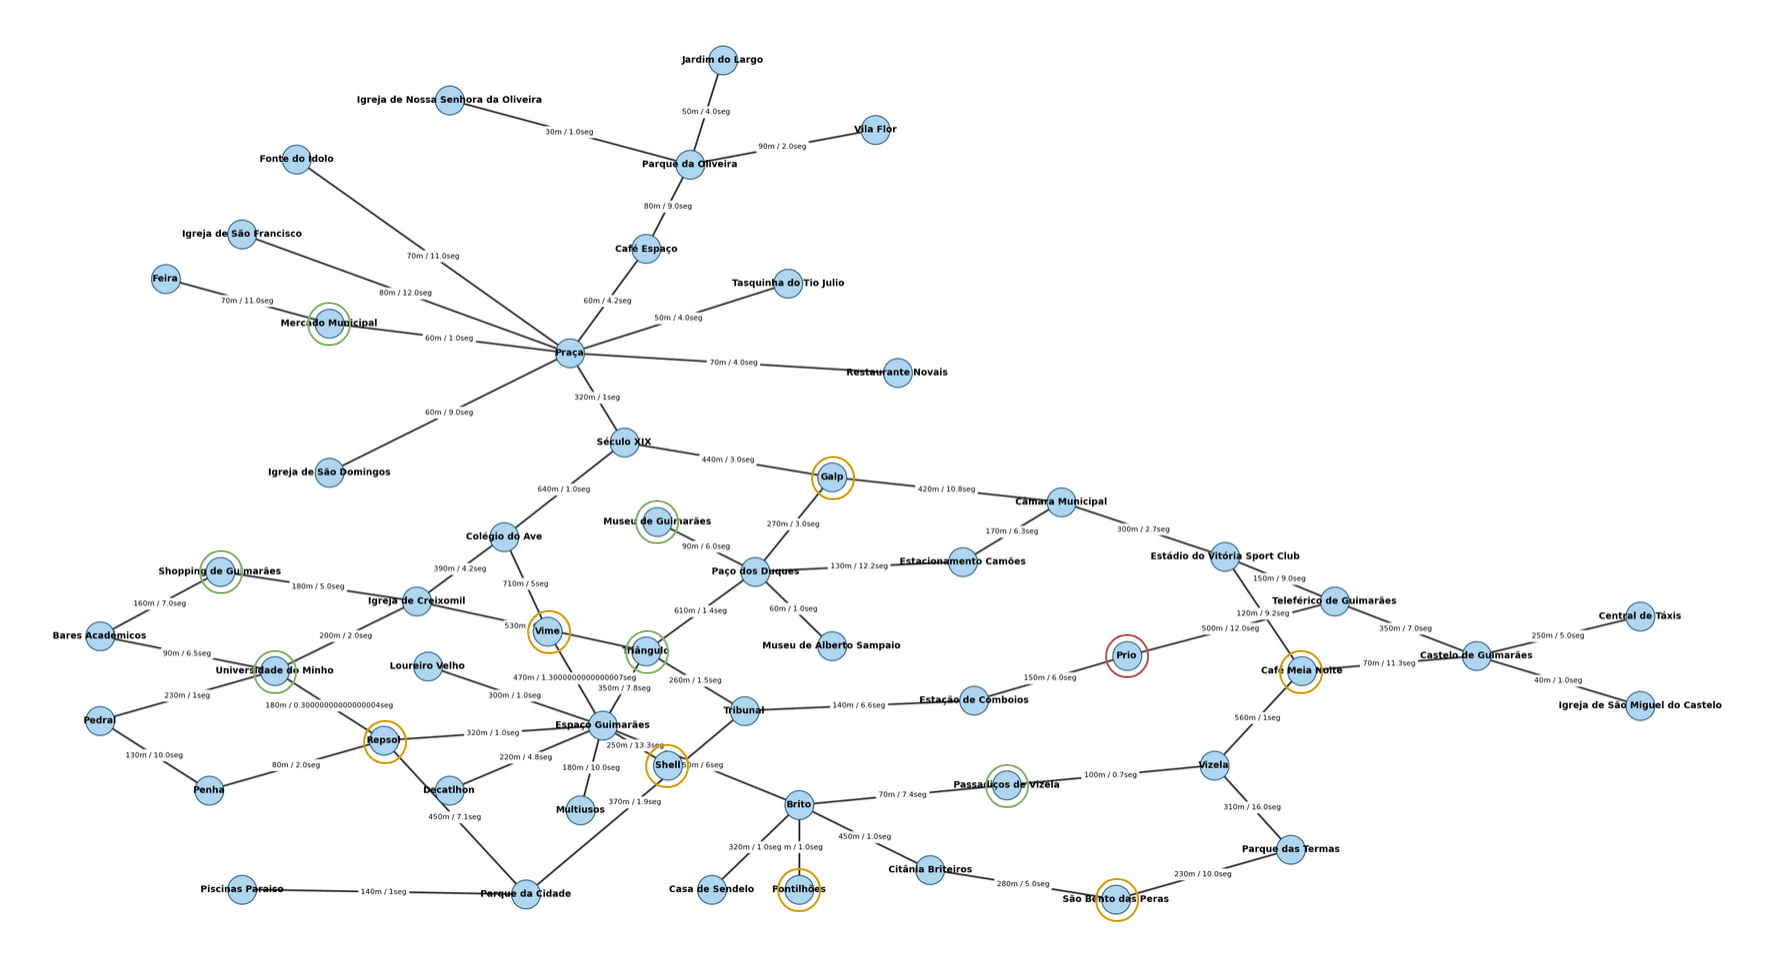
\includegraphics[width=0.9\textwidth]{imgs/cidade.png}
		\caption{Representação da cidade de Guimarães.}
		\vspace{0.2cm}
		\footnotesize
		\begin{minipage}{0.85\textwidth}
			\textbf{Legenda:}
			Círculos a verde — postos de recarga elétrica;
			Círculos a laranja — bombas de combustível;
			Círculos a vermelho — localizações com ambas as funcionalidades.
		\end{minipage}
		\label{fig:cidade}
	\end{figure}
	
	
	
	O grafo é composto por mais de 50 nodos (localizações) e as respetivas arestas (vias de circulação). Embora \textbf{todas} as localizações funcionem como pontos de recolha e entrega de passageiros, um subconjunto destes nodos funciona como postos de abastecimento:\begin{itemize}
		\item \textbf{Postos de Recarga Elétrica:} Locais como "Universidade do Minho", "Shopping de Guimarães" e "Prio", equipados com um número limitado de lugares de carregamento.
		\item \textbf{Bombas de Combustível:} Locais como "Galp", "Repsol" e "Shell", destinados ao reabastecimento dos veículos convencionais.
	\end{itemize}
	
	As arestas que conectam estes nós possuem pesos duplos — distância (metros) e tempo (segundos) — permitindo o cálculo de custos operacionais e temporais distintos.
	
	\subsection{Caraterização da Frota}
	
	A frota da \textit{TaxiGreen} é constituída por 20 veículos heterogéneos, divididos entre motorização elétrica e a combustão. Cada veículo possui atributos específicos que influenciam a tomada de decisão do agente gestor:
	
	\begin{itemize}
		\item \textbf{Veículos a Combustão:} Modelos como \textit{Toyota Corolla} ou \textit{Dacia Sandero}. Caracterizam-se por uma elevada autonomia (aprox. 700-800 km) e tempos de reabastecimento reduzidos (2 a 10 segundos simulados). No entanto, apresentam emissões de CO2 positivas e custos operacionais variáveis.
		
		\item \textbf{Veículos Elétricos:} Modelos como \textit{Tesla Model 3} ou \textit{BMW Serie 3}. Distinguem-se pela ausência de emissões diretas ($emissao\_CO2 = 0$). Em contrapartida, possuem autonomias inferiores (aprox. 300-500 km) e exigem tempos de imobilização superiores para recarga (15 a 25 segundos simulados).
	\end{itemize}
	
	Esta diversidade obriga o sistema a gerir compromissos entre a rapidez de serviço (favorecida pelos veículos a combustão em longas distâncias) e a sustentabilidade (favorecida pelos elétricos).
	
	
	
	\section{Estratégias de Procura}
	
	A navegação dos veículos no grafo da cidade é suportada por cinco algoritmos de procura distintos, implementados na classe \texttt{Graph}. A escolha do algoritmo e da função de custo é determinada dinamicamente com base nas preferências do pedido (rapidez vs economia).
	
	\subsection{Procura Não Informada}
	
	Nesta categoria, foram implementados três algoritmos que exploram o espaço de estados sem estimativas sobre a distância ao objetivo.
	
	\begin{itemize}
		\item \textbf{Breadth-First Search (BFS) e Depth-First Search (DFS):}
		Ambas as estratégias exploram o grafo com base na conectividade topológica, ignorando os pesos das arestas. A implementação do BFS utiliza uma estrutura de fila (\texttt{Queue}) para garantir a descoberta do caminho com menor número de nós, enquanto o DFS utiliza uma pilha (\texttt{stack}).
		
		\item \textbf{Uniform Cost Search (UCS):}
		Este algoritmo expande o nó com o menor custo de caminho acumulado $g(n)$, utilizando uma fila de prioridade (\texttt{heapq}). A principal particularidade desta implementação reside na definição dinâmica da função de custo $g(n)$, que varia consoante a preferência do cliente:
		\begin{itemize}
			\item Se \texttt{LOW\_COST}: $g(n)$ corresponde à distância acumulada (em metros).
			\item Se \texttt{FAST}: $g(n)$ corresponde ao tempo de viagem acumulado (em segundos), incorporando as penalizações de trânsito geradas dinamicamente.
		\end{itemize}
	\end{itemize}
	
	\subsection{Procura Informada}
	
	Para orientar a procura na direção do objetivo e melhorar a eficiência, foram implementados algoritmos que utilizam uma função heurística $h(n)$.
	
	\paragraph{Função Heurística}
	Para ambos os algoritmos informados, definiu-se como heurística admissível a \textbf{Distância Euclidiana} entre as coordenadas do nó atual ($x_n, y_n$) e as coordenadas do nó destino ($x_d, y_d$), calculada pelo método \texttt{get\_heuristic}:
	\[ h(n) = \sqrt{(x_d - x_n)^2 + (y_d - y_n)^2} \]
	Esta métrica estima a distância em linha reta, garantindo que nunca sobrestima o custo real em termos de distância.
	
	\begin{itemize}
		\item \textbf{Greedy Search:}
		Seleciona o próximo nó a expandir baseando-se exclusivamente na minimização de $h(n)$. A implementação mantém uma \texttt{open\_list} e seleciona iterativamente o vizinho que apresenta a menor distância euclidiana ao destino, ignorando o custo do trajeto já percorrido.
		
		\item \textbf{A* (A-Star):}
		Combina o custo real do caminho com a estimativa heurística, minimizando a função de avaliação $f(n) = g(n) + h(n)$.
		Tal como no UCS, o componente $g(n)$ adapta-se à preferência do pedido (tempo ou distância). O algoritmo gere duas listas (\texttt{open\_list} e \texttt{closed\_list}) para assegurar que cada nó é avaliado e expandido de forma ótima, garantindo a melhor solução possível para a métrica de custo selecionada.
	\end{itemize}
	
	
	\section{Estatísticas}
	
	O agente \texttt{TaxiGreenGestor} calcula as seguintes estatísticas (exemplo apresentado na figura \ref{fig:estatisticas}):
	\begin{itemize}
		\item \textbf{Tempo Médio de Resposta}: este cálculo permite comparar os algoritmos perante a velocidade de resposta ao pedidos. Podemos verificar pela figura \ref{fig:estatisticas} que os algoritmos de procura não informados têm uma melhor performance relativamente aos algoritmos de procura informada, devendo-se ao facto de estes algoritmos não se guiarem pelos custos das ligações (exceto o de custo uniforme). O algoritmo de procura em profundidade tem melhores resultados como é verificável.
		\item \textbf{Taxa de ocupação média}: esta estatística permite analisar a percentagem de veículos ocupados, sendo registada a cada 10 segundos e calculada a média no fim. Todos os algoritmos aparentam ter uma performance uniforme nesta estatística.
		\item \textbf{Custo Operacional}: este gráfico indica o custo operacional total de cada algoritmo, e podemos verificar que o algoritmo de procura em profundiadde tem resultados piores, dado que é mais provável que o caminho seja mais profundo, comparado a outros algoritmos.
		\item \textbf{Emissão de CO2}: esta estatística apresenta as emissões de CO2 totais, e mais uma vez a procura em profundidade falha em comparação aos outros algoritmos.
		\item \textbf{Metros sem passageiros}: este cálculo permite comparar os algoritmos sobre a distância percorrida sem passageiros. O algoritmo de procura em profundidade, mais uma vez, tem uma performance má, pois tem a tendência a calcular caminhos mais longos, percorrendo maiores distâncias.
		\item \textbf{Média de lugares vazios}: esta estatística apresenta a percentagem média de lugares vazios nos veículos. Podemos verificar que todos os algoritmos têm valores semelhantes, dado que não foi criado nenhuma gestão relativa aos lugares ocupados.
		\item \textbf{Número de pedidos rejeitados}: esta estatística apresenta o número de pedidos rejeitados, e podemos verificar que num total de 100 pedidos, nenhum foi rejeitado, ou seja, todos os algoritmos conseguiram resolver todos os pedidos.
		\item \textbf{Número de carros bloqueados}: este gráfico apresenta o número de veículos que ficaram bloqueados, isto é, chegaram a um nível de autonomia que não os permite alcançar nenhum posto de recarga ou bomba de combustível. Nenhum veículo ficou bloqueado, logo temos uma boa gestão por parte do agente.
	\end{itemize}
	
	\begin{figure}[h]
		\centering
		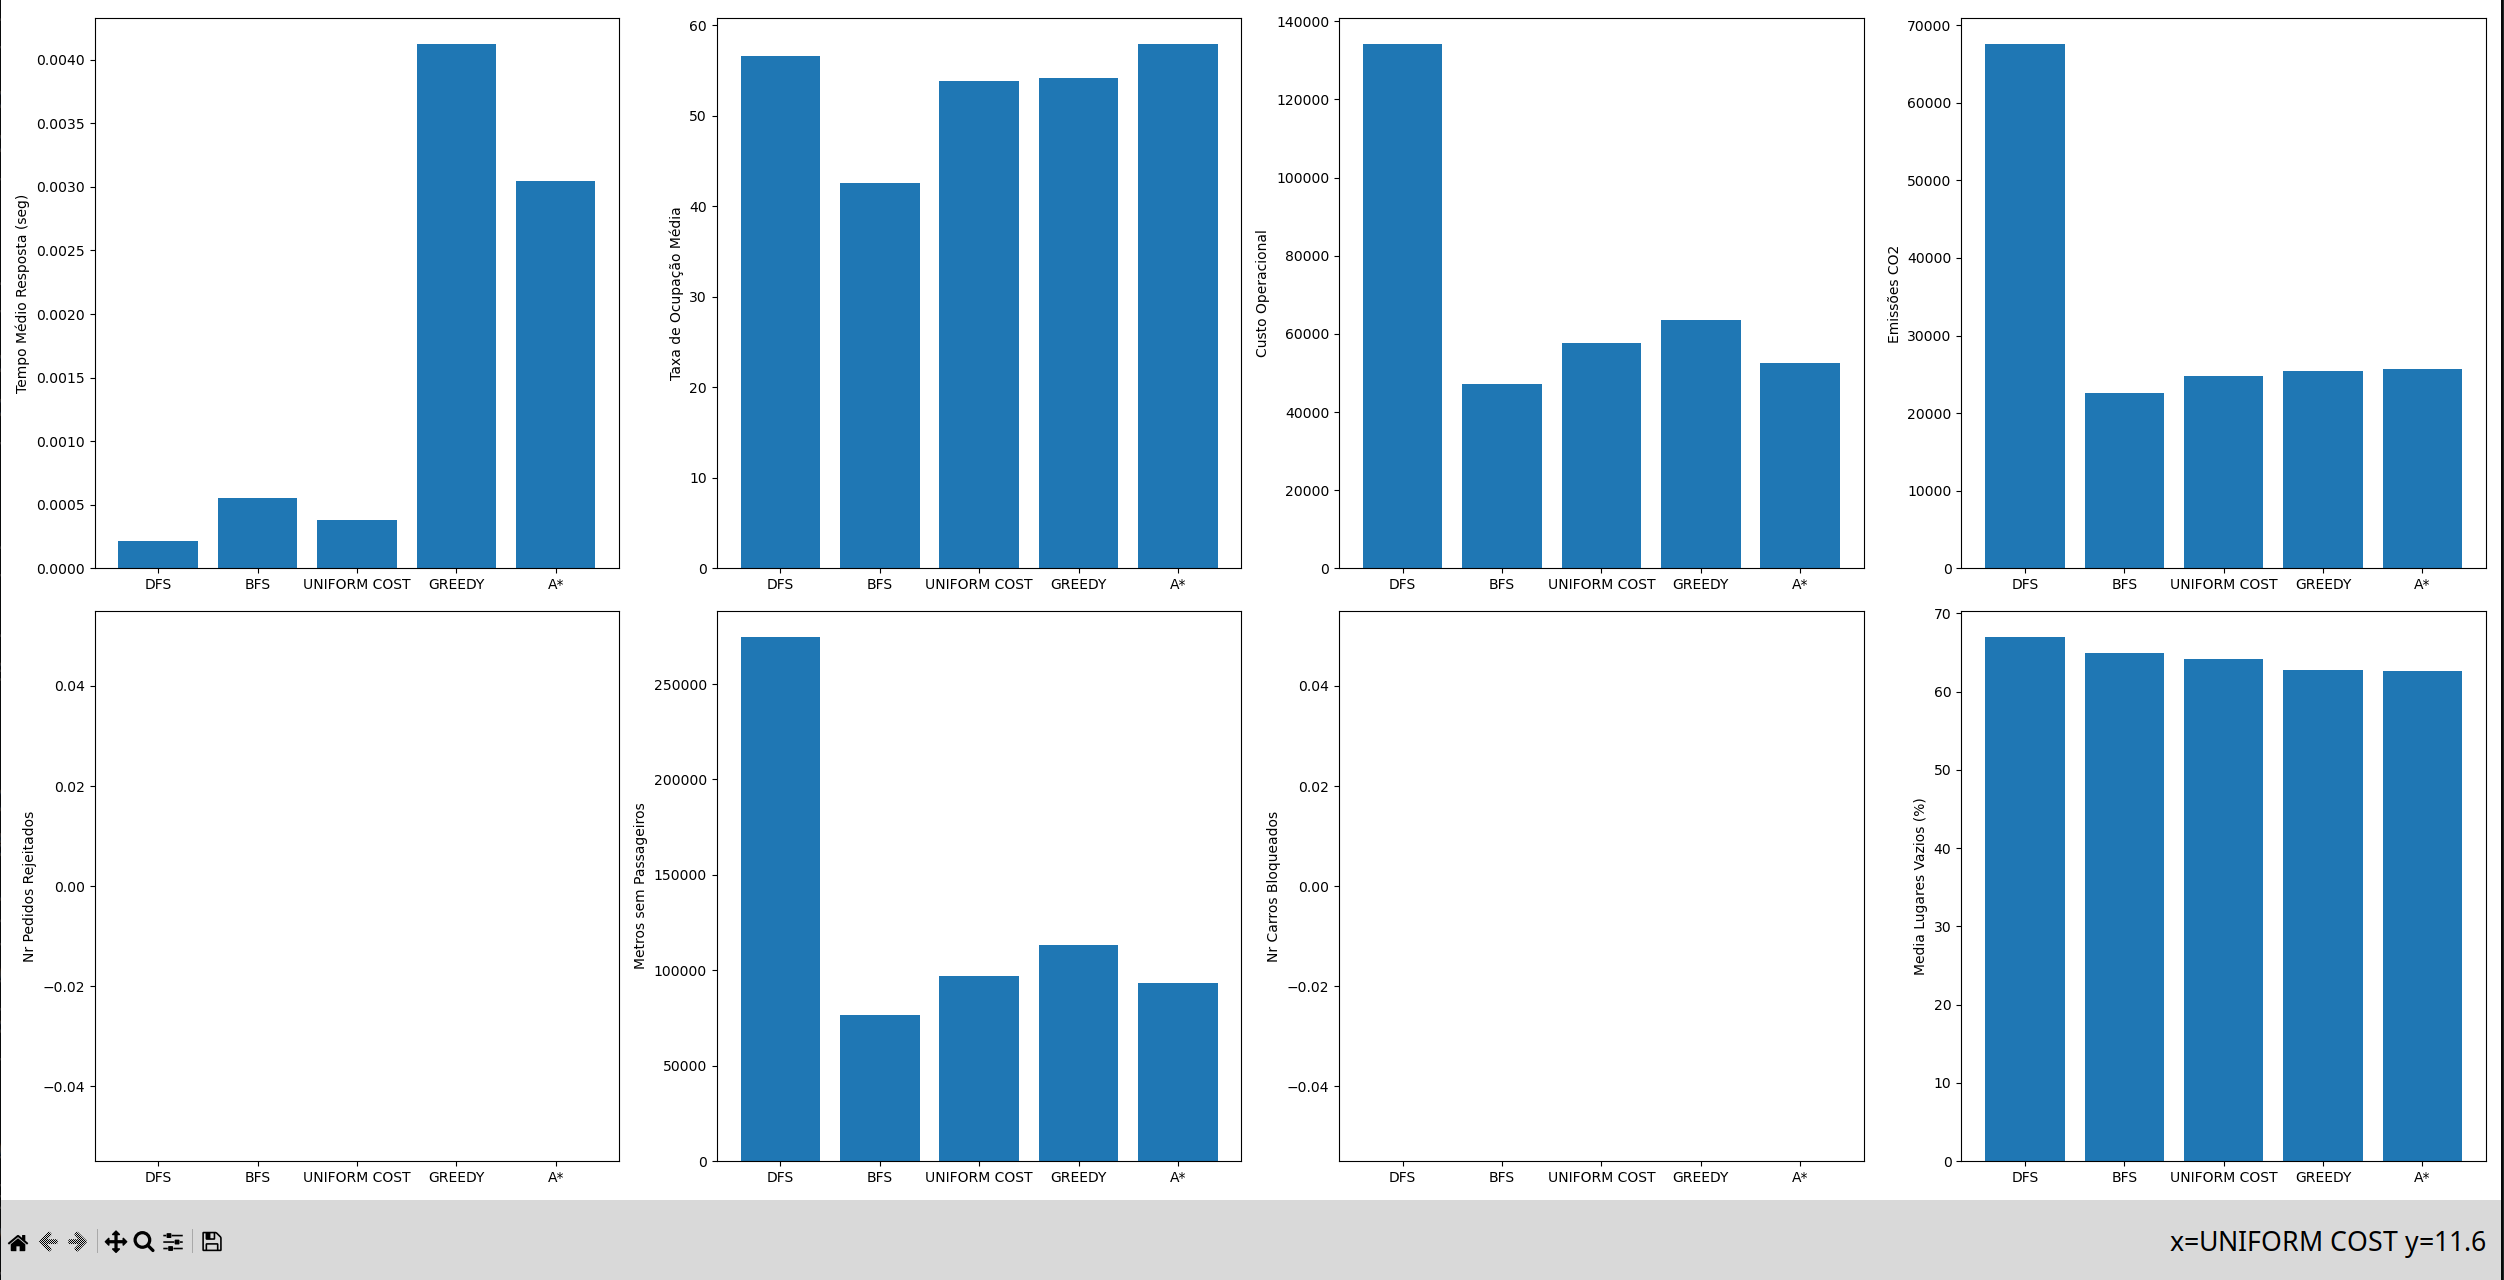
\includegraphics[width=1\linewidth]{imgs/estatisticas.png}
		\caption{Estatísticas}
		\label{fig:estatisticas}
	\end{figure}
	
	É importante realçar que os pedidos realizados pelos algoritmos são aleatórios e diferentes, isto é, um algoritmo nunca irá resolver os mesmos pedidos que outro algoritmo, logo não é possível comparar os algoritmos em detalhe, mas de forma global podemos observar certas diferenças. Um exemplo disso é o algoritmo de procura em profundidade, que embora seja rápido a responder pedidos, as rotas calculadas são longas, obtendo custos elevados.
	
	\section{Conclusão}
	
	Neste trabalho prático foi desenvolvido um sistema inteligente para a gestão e otimização de uma frota de táxis mista (elétricos e a combustão) na cidade de Guimarães. A implementação permitiu aplicar conceitos fundamentais de Inteligência Artificial, nomeadamente a aplicação de algoritmos de procura em grafos, a utilização de heurísticas e a modelação de ambientes dinâmicos.
	
	A estrutura do sistema, controlada pelo\texttt{TaxiGreenGestor}, permitiu coordenar múltiplos veículos e pedidos concorrentes de forma eficiente. A modelação da cidade como um grafo ponderado, distinguindo custos temporais e espaciais, garantiu flexibilidade ao sistema, possibilitando a otimização de rotas segundo critérios distintos (rapidez ou economia) num mesmo ambiente operacional.
	
	Decisões como a adoção da distância euclidiana como heurística admissível e a gestão proativa da autonomia provaram ser essenciais para viabilizar a operação da frota elétrica sem comprometer a disponibilidade do serviço. A estratégia de reabastecimento dinâmico permitiu mitigar as limitações de alcance dos veículos elétricos.
	
	Apesar da eficácia demonstrada, o sistema atual realiza uma alocação exclusiva de um veículo por pedido. Como melhoria futura, sugere-se a implementação de um mecanismo de \textit{ride-sharing}, permitindo que o mesmo veículo transporte passageiros de pedidos distintos com rotas compatíveis, o que aumentaria significativamente a taxa de ocupação e a eficiência global da frota.

\end{document}
